\chapter{Plataformas}
\label{chap:Plataformas}

Para a localização com os resíduos de comunicação \emph{Wi-Fi} são necessários
sensores que possam capturar estes resíduos e processar qualquer informação
capturada pelo sensor deste trabalho. Esta plataforma de sensor pode ser construída com
qualquer plataforma computacional capaz de ser programada com comunicação
\emph{Wi-Fi}, porém o \emph{hardware} de \emph{Wi-Fi} e seu \emph{software}
controlador deve permitir o Modo Promíscuo.

Este Modo Promíscuo (\emph{promiscuous mode}) é definindo pela capacidade de uma
Placa Adaptadora de Rede \emph{Wi-Fi} (\emph{Network Interface Card} -
\emph{NIC}) receber e interpretar todos os pacotes que trafegam em uma rede ou
em todas as redes que estão em seu alcance, independentemente do destinatário do
pacote. Em seu funcionamento normal, uma \emph{NIC} descarta todos os pacotes que
não são destinados para ela o mais cedo possível, evitando reprocessamento de
dados indesejáveis, por este motivo não são todas as \emph{NICs} que permitem o
Modo Promíscuo. Essa funcionalidade elimina a necessidade de \emph{hardware} ou
\emph{software} em cada um dos dispositivos rastreados.

Neste sentido, elegeu-se duas plataformas de notável importância no mercado atual
e notável facilidade de acesso para qualquer interessado na área. As plataformas
testadas foram o microcomputador \emph{Raspberry Pi} e o microcontrolador
\emph{ESP8266}. Ambos  foram escolhidos pelo domínio do segmento de Prototipação
e Faça Você Mesmo  (\emph{Do It Yourself} - \emph{DIY}) dentro do campo de IoT.
Outro líder de segmento, o \emph{Arduino}  foi prontamente descartado por não
conter nativamente a habilidade de conectar-se à \emph{Internet} sendo
constantemte combinado com um dos escolhidos para ganhar esta habilidade,
demonstrando claramente menor afinidade a este projeto em comparação aos seus
igualmente famosos concorrentes.

Após escolhidas as plataformas de intersse alguns exemplares de cada uma delas
foi adquirido para implementar a aplicação proposta. Neste sentido, serão
apresentadas cada uma dessas plataformas quanto as suas especificações técnicas
e aos produtos utilizados em conjunto para que elas pudessem funcionar e serem
programadas e os motivos pela adoção ou não delas.


\section{ESP8266}
\label{sec:ESP8266}

O ESP8266 é um SOC (\emph{System On a Chip} - Sistema em um \emph{Chip}),
ou seja, é um chip com todos os componentes lógicos
eletrônicos necessários e partes para um dado sistema em único cirtuito
integrado. Este chip possui:


\begin{alineas}
	\item \emph{Wi-Fi} embutido com capacidade de 2,4 GHz (802.11 b/g/n);

	\item 16 GPIOs (\emph{general-purpose input/output}) incluindo interfaces
 I2U, SPI, UART, entrada ADC, saída PWM;

	\item Arquitetura \emph{RISC} de 32 bits;

	\item CPU que opera em  80 MHz, com possibilidade de operar em 160 MHz;

	\item 64 KB de ROM para \emph{boot};

	\item 64 KB de RAM para instruções;

	\item 96 KB de RAM para dados;

	\item Memória \emph{Flash SPI} de 512 KB a 4 MB (dependente de módulo externo);

	\item Núcleo baseado no \emph{IP Diamand Standard LX3} da \emph{Tensilica}.

\end{alineas}

Para o mercado de prototipação, fabricantes constroem placas de diferentes configurações com
este chip como elemento central, os chamados módulos. Estes módulos usam o
ESP8266 com diferenças perceptíveis, por exemplo, quantidade de pinos, dimensões
físicas e alguns podem até operar de modo \emph{standalone} (sem outro \emph{hardware} de
suporte como reguladores de tensão, conversores serial-USB) e especialmente a
 \emph{Memória Flash SPI}. Neste trabalho, foram usados os módulos:
\emph{ESP-01}, \emph{LoLin}, \emph{D1 mini} e \emph{ESP-12F} com placa adaptadora de pinos.


\begin{figure}[htb]
	\caption{\label{fig:modelos-esp}Módulos ESP8266}
	\begin{center}
		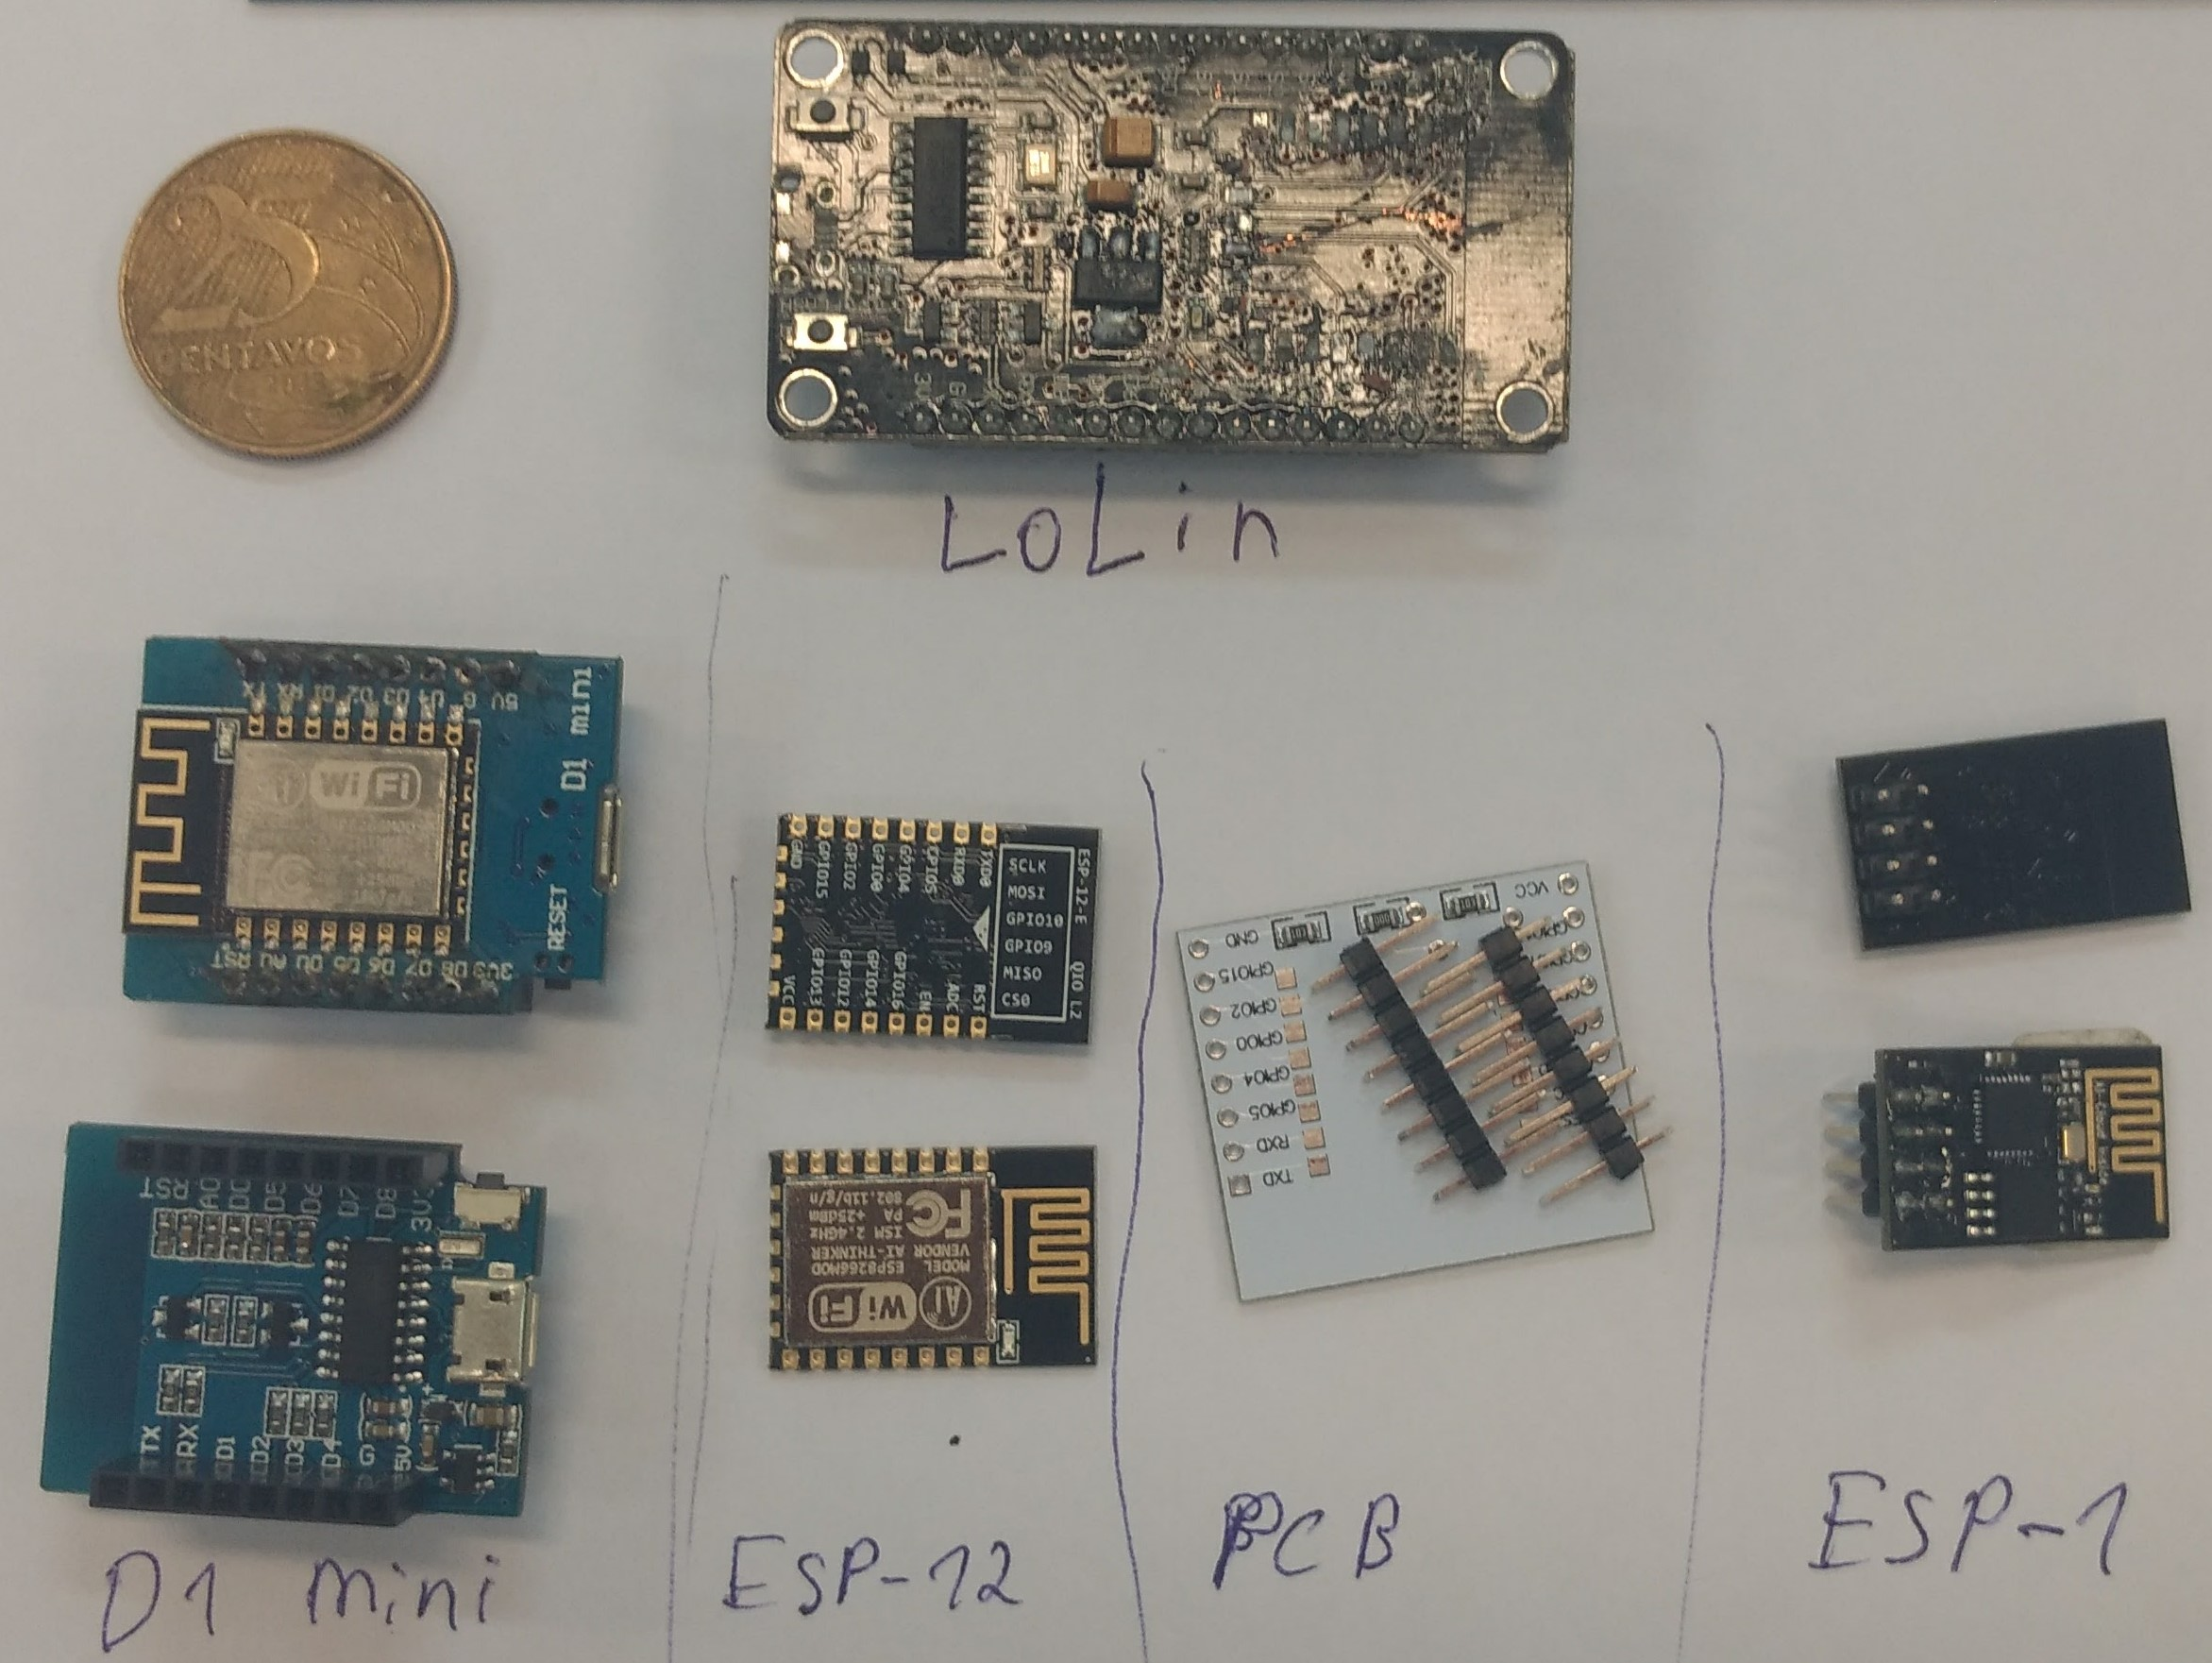
\includegraphics[width=1\textwidth]{040-plataformas/esp-dev/modulos-esp.jpg}
	\end{center}
	\legend{Fonte: Elaborada pelo autor}
\end{figure}



\subsection{Disponibilidade no mercado}
\label{subsec:mercado-esp}

As diferentes especificações implicam em diferentes produtos e mercado para
eles, isto resulta em diferentes preços em diferentes regiões.

\begin{table}[htb]
\IBGEtab{%
\ABNTEXchapterfont {
  \caption{Descrição de custos de módulos ESP8266}%
  \label{table:custo-esp}
}
}{%
\begin{tabular}{cccc}
	\toprule
	Módulo				&	N° de pinos		&	Memória	&	Preço			\\
	\midrule \midrule
	ESP-01				&	8				&	1 MB	&	R\$ 16,80 		\\
	\midrule
	ESP-12F				&	22				&	4 MB	&	R\$ 14,90 		\\
	\midrule
	PCB (sem ESP-12F)	&	16				&	4 MB	&	R\$ 3,45 		\\
	\midrule
	D1 mini (ESP-12F)	&	16 + microUSB	&	4 MB	&	R\$ 12,56^{1}	 	\\
	\midrule
	LoLin (ESP-12F)		&	30 + microUSB	&	4 MB	&	R\$ 35,87 		\\
	\midrule
	\bottomrule
\end{tabular}%
}{%
	\fonte{Produzido pelo autor.}%
	\nota[Nota 1]{D1 mini (ESP-12F) foi adquirido do mercado chinês.}%
}
\end{table}

A escolha do ESP8266 como primeira tentativa devido o seu baixo custo e de
tamanho reduzido. No exterior, ele pode ser encontrado por de
USD \$1.76 a 2.2 \citeonline{Alibaba}, e no
Brasil, em média, por R\$ 15,00 \citeonline{mercadoLivre}.

Devido ao seu tamanho, ele é de fácil integração com demais dispositivos,
bastando o uso de uma comunicação serial. Já sobre a comunidade, há inúmeros
projetos DIY (em inglês \emph{do it yourself}, em português "faça você mesmo") que
ensinam a como construir e manipular projetos que envolvem diferentes módulos.
Além disso, a empresa  idealizadora e fabricante do chip, Espressif,
disponibiliza no GitHub projetos com documentação e código aberto.

Para desenvolver na plataforma, os módulos ESP foram utilizados de formas
diferentes dependendo das capacidades de cada módulo.
Quando o módulo
possuía regulador de tensão embarcado, utilizava-se o próprio conectado a uma
porta USB. Quando o módulo não possuía tal, utilizava-se um circuito com fonte
externa (pilhas ou USB) e um regulador de tensão conectados aos pinos \emph{3v3} e \emph{GND}.
Depedendo da complexidade do circuito para ligar e ter acesso à serial do
módulo, é necessário o uso de uma placa \emph{breadboard}, como na \autoref{fig:esp-pilha-serial}.
Para este trabalho foi utilizado o regular \emph{AMS1117 3v3} e dois capacitores de 100 \mu F.

\begin{figure}[htb]
	\caption{\label{fig:esp-pilha-serial}ESP-12F com regulador tensão e serial}
	\begin{center}
		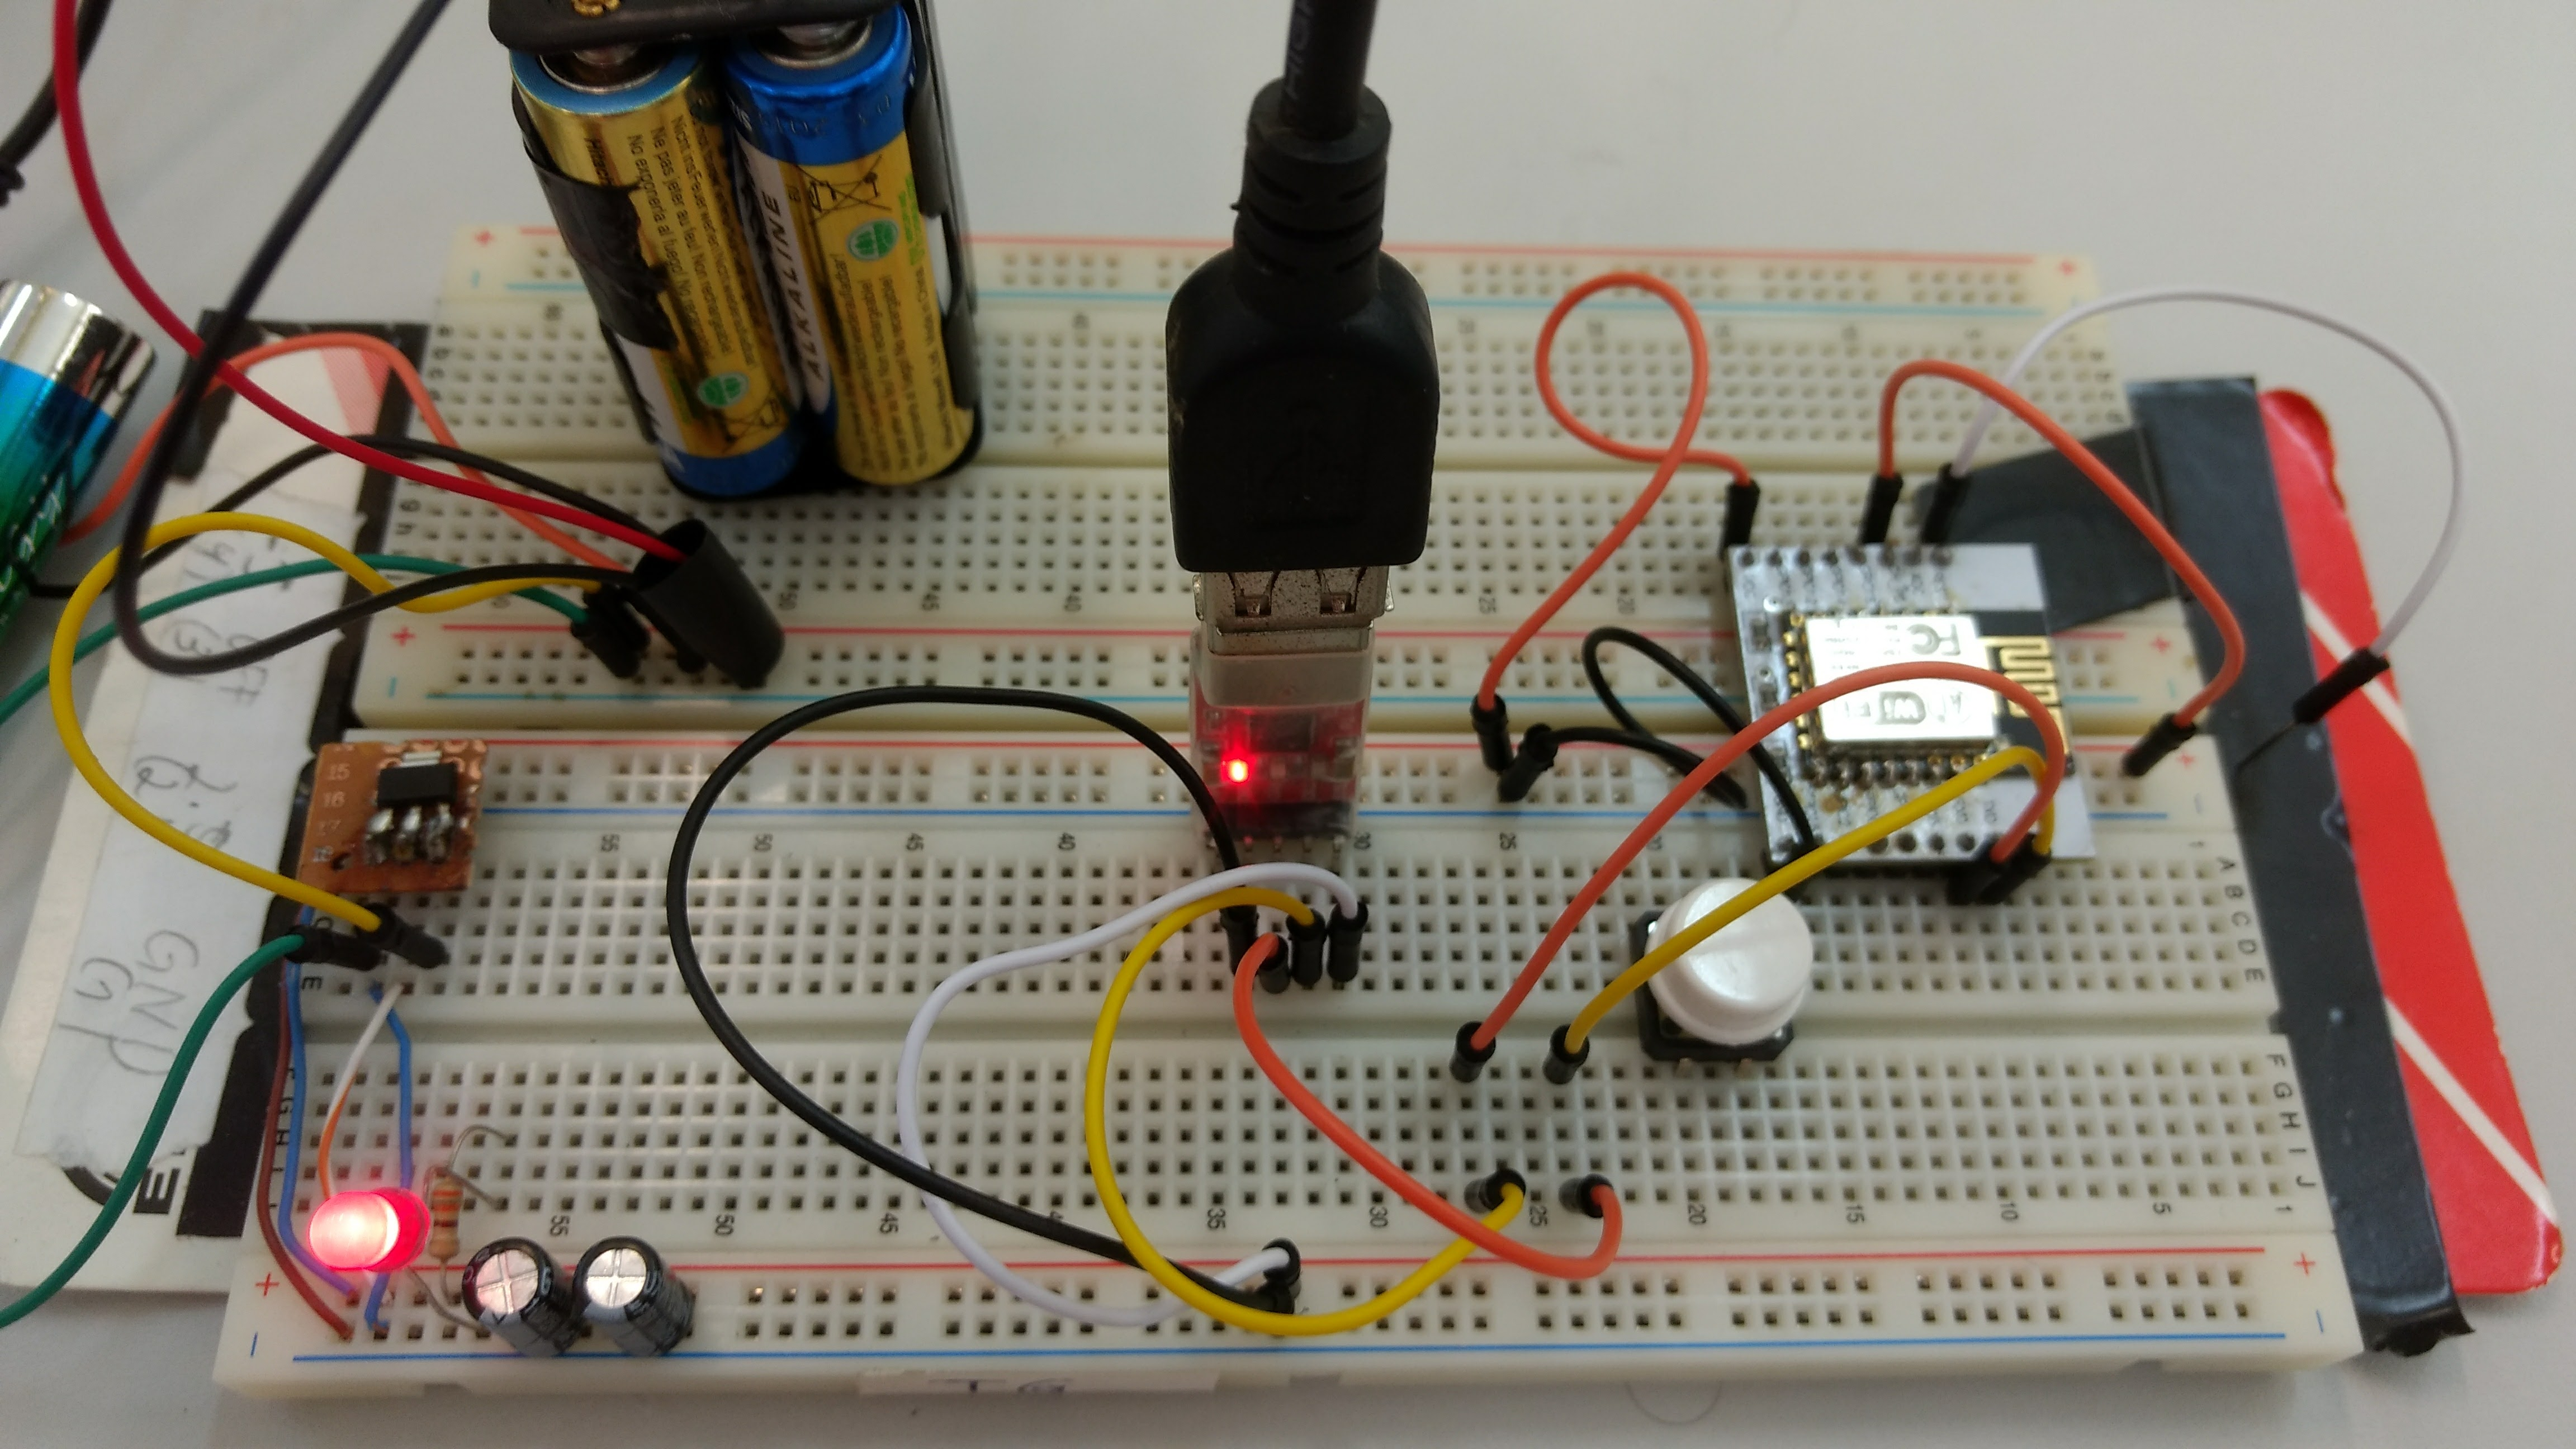
\includegraphics[width=1\textwidth]{040-plataformas/esp-dev/breadboard.jpg}
	\end{center}
	\legend{Fonte: Elaborada pelo autor}
\end{figure}


\subsection{Desenvolvimento e Implantação}
\label{subsec:dev-esp}

Todo código produzido em uma linguagem de programação é compilado por uma
ferramenta e, então, carrega-se os arquivos binários para o ESP8266 através da
serial, para que a execução do código seja iniciada. Na \autoref{fig:esp-toolchain}, é
apresentado um modelo de desenvolvimento e implantação desde o código até chegar
no módulo ESP e, também, a lista de carregadores usados.

\begin{verbatim}
+--------+           +-----------+
| Código |-----------> Compilador|
+--------+           |           |      +----------------------+
                     |  Ligador  <------| Cabeçalhos Espressif |
                     +-----------+      +----------------------+
                           |
+------------+        +----v-----+
| Carregador <--------+ Binários |
+-----+------+        +----------+
       \
        \---Serial
         \
+---------v----+
|  Módulo ESP  |
+--------------+
\end{verbatim}



\begin{table}[htb]
\IBGEtab{%
\ABNTEXchapterfont {
	\caption{Ferramentas para desenvolvimento com ESP8266}%
	\label{table:tools-esp}
}
}{%
\begin{tabular}{cccc}
	\toprule
	Ferramenta			&	Editor	&	Compilador e Ligador	&	Carregador	\\
	\midrule \midrule
	Arduino IDE			&	Sim		&	arduino C				&	Sim, mas não carrega binários pré compilados	\\
	\midrule
						&			&	NodeMCU Lua,			&		\\
	ESPlorer			&	Sim		&	MicroPython,			&	Não, conta com firmware específico	\\
						&			&	AT e RN2483				&		\\
	\midrule
	esptool.py			&	Não		&	Não 					&	Somente binários pré compilados	\\
	\midrule
	ESP8266 Flash		&			&							&		\\
	Downloader			&	Não		&	Não 					&	Somente binários pré compilados	\\
	\midrule
	NodeMCU Firmware	&			&							&		\\
	Programmer			&	Não		&	Não 					&	Somente binários pré compilados	\\
	\midrule
	\bottomrule
\end{tabular}%
}{%
	\fonte{Produzido pelo autor.}%
}
\end{table}

Todo código produzido é carregado para o módulo ESP através de seu barramento
serial. Alguns modelos, como o \emph{LoLin} e \emph{D1 mini}, já apresentam conversor serial
para \emph{micro-USB}. Para os que não possuem tal interface é necessário utilizar um
conversor serial-USB externo, a \selfef{fig:esp-pilha-serial} demonstra esse método.

As \emph{GPIOs} do \emph{ESP-12F} são acessadas somente através de placas
de circuito impresso, então uma foi adquirida para a programação do mesmo.

Dos conversores serial-USB adquiridos, o modelo \emph{CH340G} não funcionou por
não ter driver compatível com o \emph{Windows 10}, em contraste com o modelo
\emph{CP2102}  que funcionou no mesmo sistema operacional.


\subsection{Testes e resultados}
\label{subsec:mercado-esp}

O primeiro objetivo durante a programação dos módulos ESP8266 é cumprir a
premissa  estabelecida no início deste capítulo de acessar o Modo Promíscuo da
interface Wi-Fi. Neste caso, procurou-se pelo ponto da \emph{API} de
\emph{hardware} do ESP8266 onde os pacotes destinados a outros dispositivos são
descartados, desativar este filtro, capturar e avaliar o pacote para localizar o
seu emissor.

A principio, com o \emph{firmware AT} que é o padrão do módulo ESP-01 e com o
emulador de serial da \emph{Arduino IDE} ou a aplicação \emph{Cool Term} é
possível configurar e utilizar o módulo por completo apenas com instuções AT
enviadas através da conexão serial. A primeira investigação sobre a API do protocolo
AT indicou \citeonline{room15} como a fonte mais completa sobre as capacidades
do \emph{firmware AT} e não revelou nenhuma capacidade de ativar o Modo Promíscuo.

Também utilizou-se a linguagem C que foi compilada na \emph{Arduino IDE} e
enviada ao ESP8266 com a extenção \emph{esp8266 by ESP8266 Community} que inclui
os cabeçalhos de funções para que o compilador padrão da \emph{Arduino IDE} gere
código  executável pelo ESP8266. Mesmo nesta API, nenhuma capacidade de ativar o
Modo Promíscuo foi encontrada.

\begin{figure}[htb]
	\caption{\label{fig:esp-arduino}Código em C compilado e implantado em um ESP8266}
	\begin{center}
		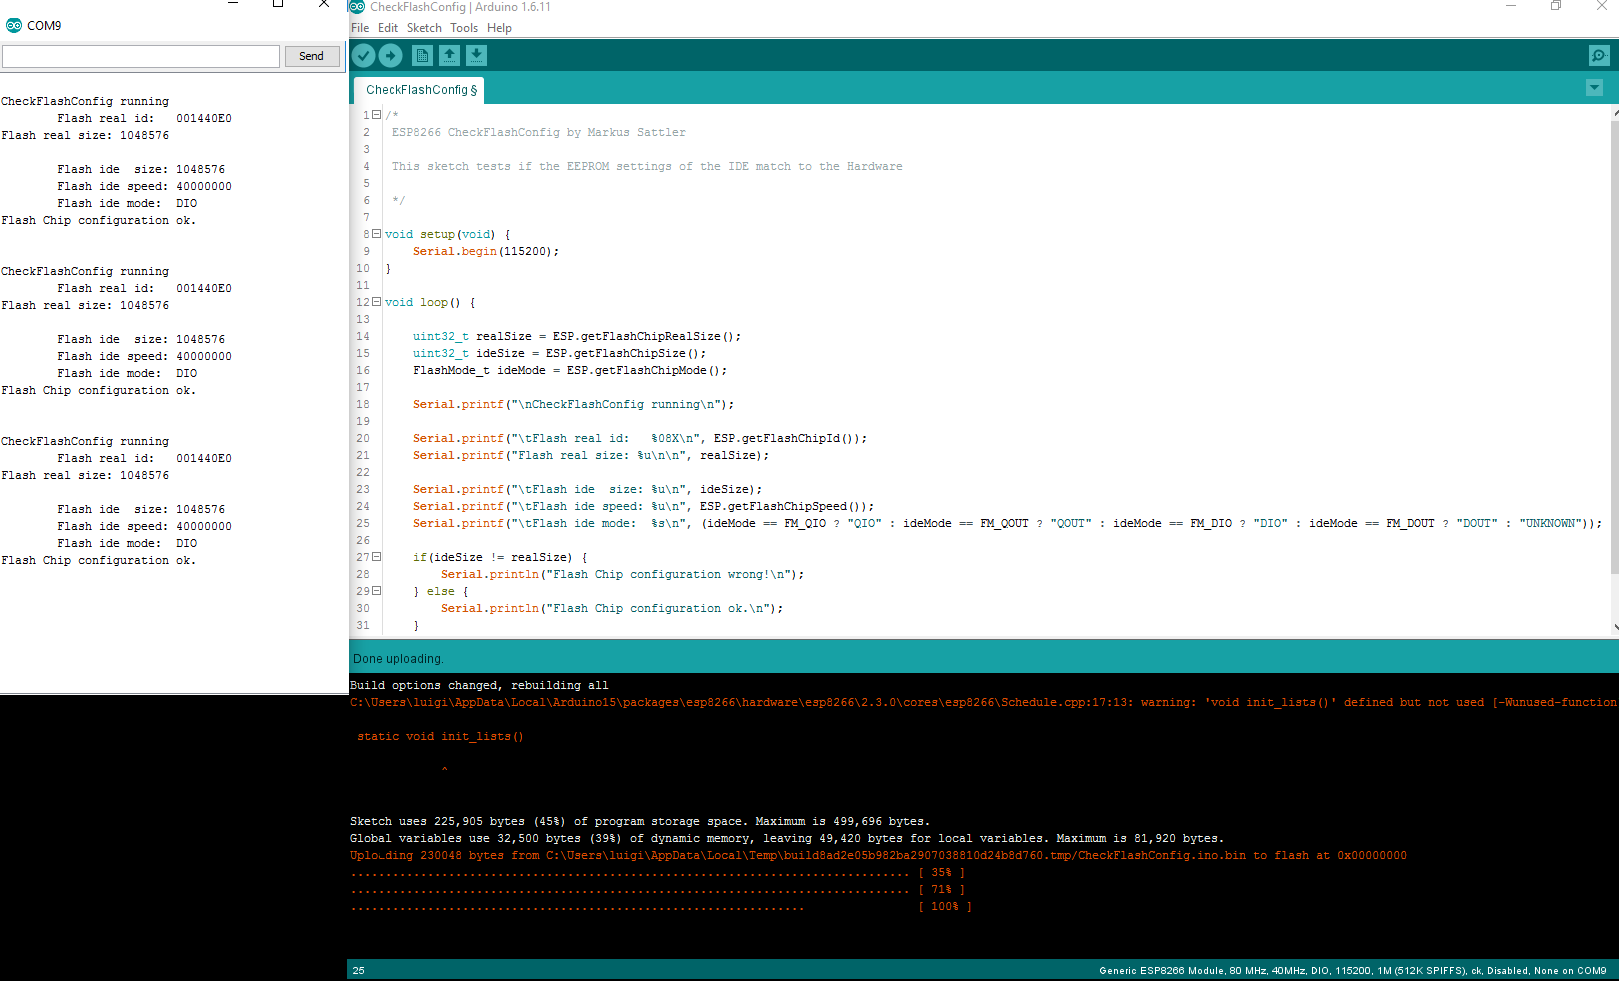
\includegraphics[width=1\textwidth]{040-plataformas/esp-dev/arduino-ide.png}
	\end{center}
	\nota[Esquerda]{Comandos AT no emulador de serial da \emph{Arduino IDE}.}%
	\nota[Direita]{Editor da \emph{Arduino IDE} com código C.}%
	\nota[Abaixo em preto]{Processo de \emph{upload} do firmware escrito em C.}%
	\fonte{Elaborado pelo autor.}%
\end{figure}


Nova tentativa para a programação  dos módulos escolhidos foi feita através de
\emph{toolchains} (conjunto de ferramentas para desenvolvimento de software) da
empresa \emph{Espressif} e de um usuário do \emph{Github}, muito utilizado para
projetos de ESPs, Paulo Sokolovsky (\cite{Pfalcon}). Ambas as \emph{toolchains}
são \emph{SDKs} de código aberto. Os \emph{scripts} foram feitos na linguagem C,
compilados nessas SDKs e transferidos para os módulos ESP. Neste caso,
a configuração delas mostrou-se um desafio pois requisitavam uma versão
específica do \emph{Ubuntu Linux} que a máquina utilizada para o desenvolvimento
não suporta. Também foi testada a utilização de máquinas virtuais mas, novamente,
a máquina do desenvolvedor não possui virtualização impossibilitando esta opção.

Em conclusão, apesar do baixo custo e documentação da comunidade aberta, o
ESP8266 não foi adotado como sensor, pois não foi possível colocá-lo em modo
prosmícuo, essencial para detectar pacotes entre dispositivo e os pontos de
acesso inviabilizando completamente o uso desta plataforma mesmo esta sendo a
mais adequada e promissora no ponto de vista da construção de um produto final
por seu extremo baixo custo.

\section{Raspberry Pi}
\label{sec:Raspberry-Pi}

O \emph{Raspberry PI 3 Model B} é um computador \emph{single-board}  (única
placa) que tem o tamanho próximo ao de um cartão de crédito. Foi desenvolvido
pela \emph{Raspberry Pi Foundation} para promover o ensino da computação nas escolas.
Este computador possui:


\begin{alineas}
	\item Antena \emph{Wi-Fi} embutida 802.11n;

	\item \emph{Bluetooth 4.1} e \emph{Bluetooth Low Energy} (BLE);

	\item 1 GB RAM;

	\item Processador Gráfico \emph{VideoCore IV 3D};

	\item ARM CPU de 1.2 GHz quad-core 64-bit.

	\item 4 portas USB;

	\item 40 pinos GPIOs;

	\item Porta HDMI;

	\item Porta \emph{Megabit Ethernet};

	\item Saída de aúdio e vídeo 3.5 mm;

	\item Interface para câmera (CSI) e monitor (DSI);

	\item Leitor para cartão \emph{micro SD};

\end{alineas}

\begin{figure}[htb]
	\caption{\label{fig:rpi-3}Raspiberry Pi 3 }
	\begin{center}
		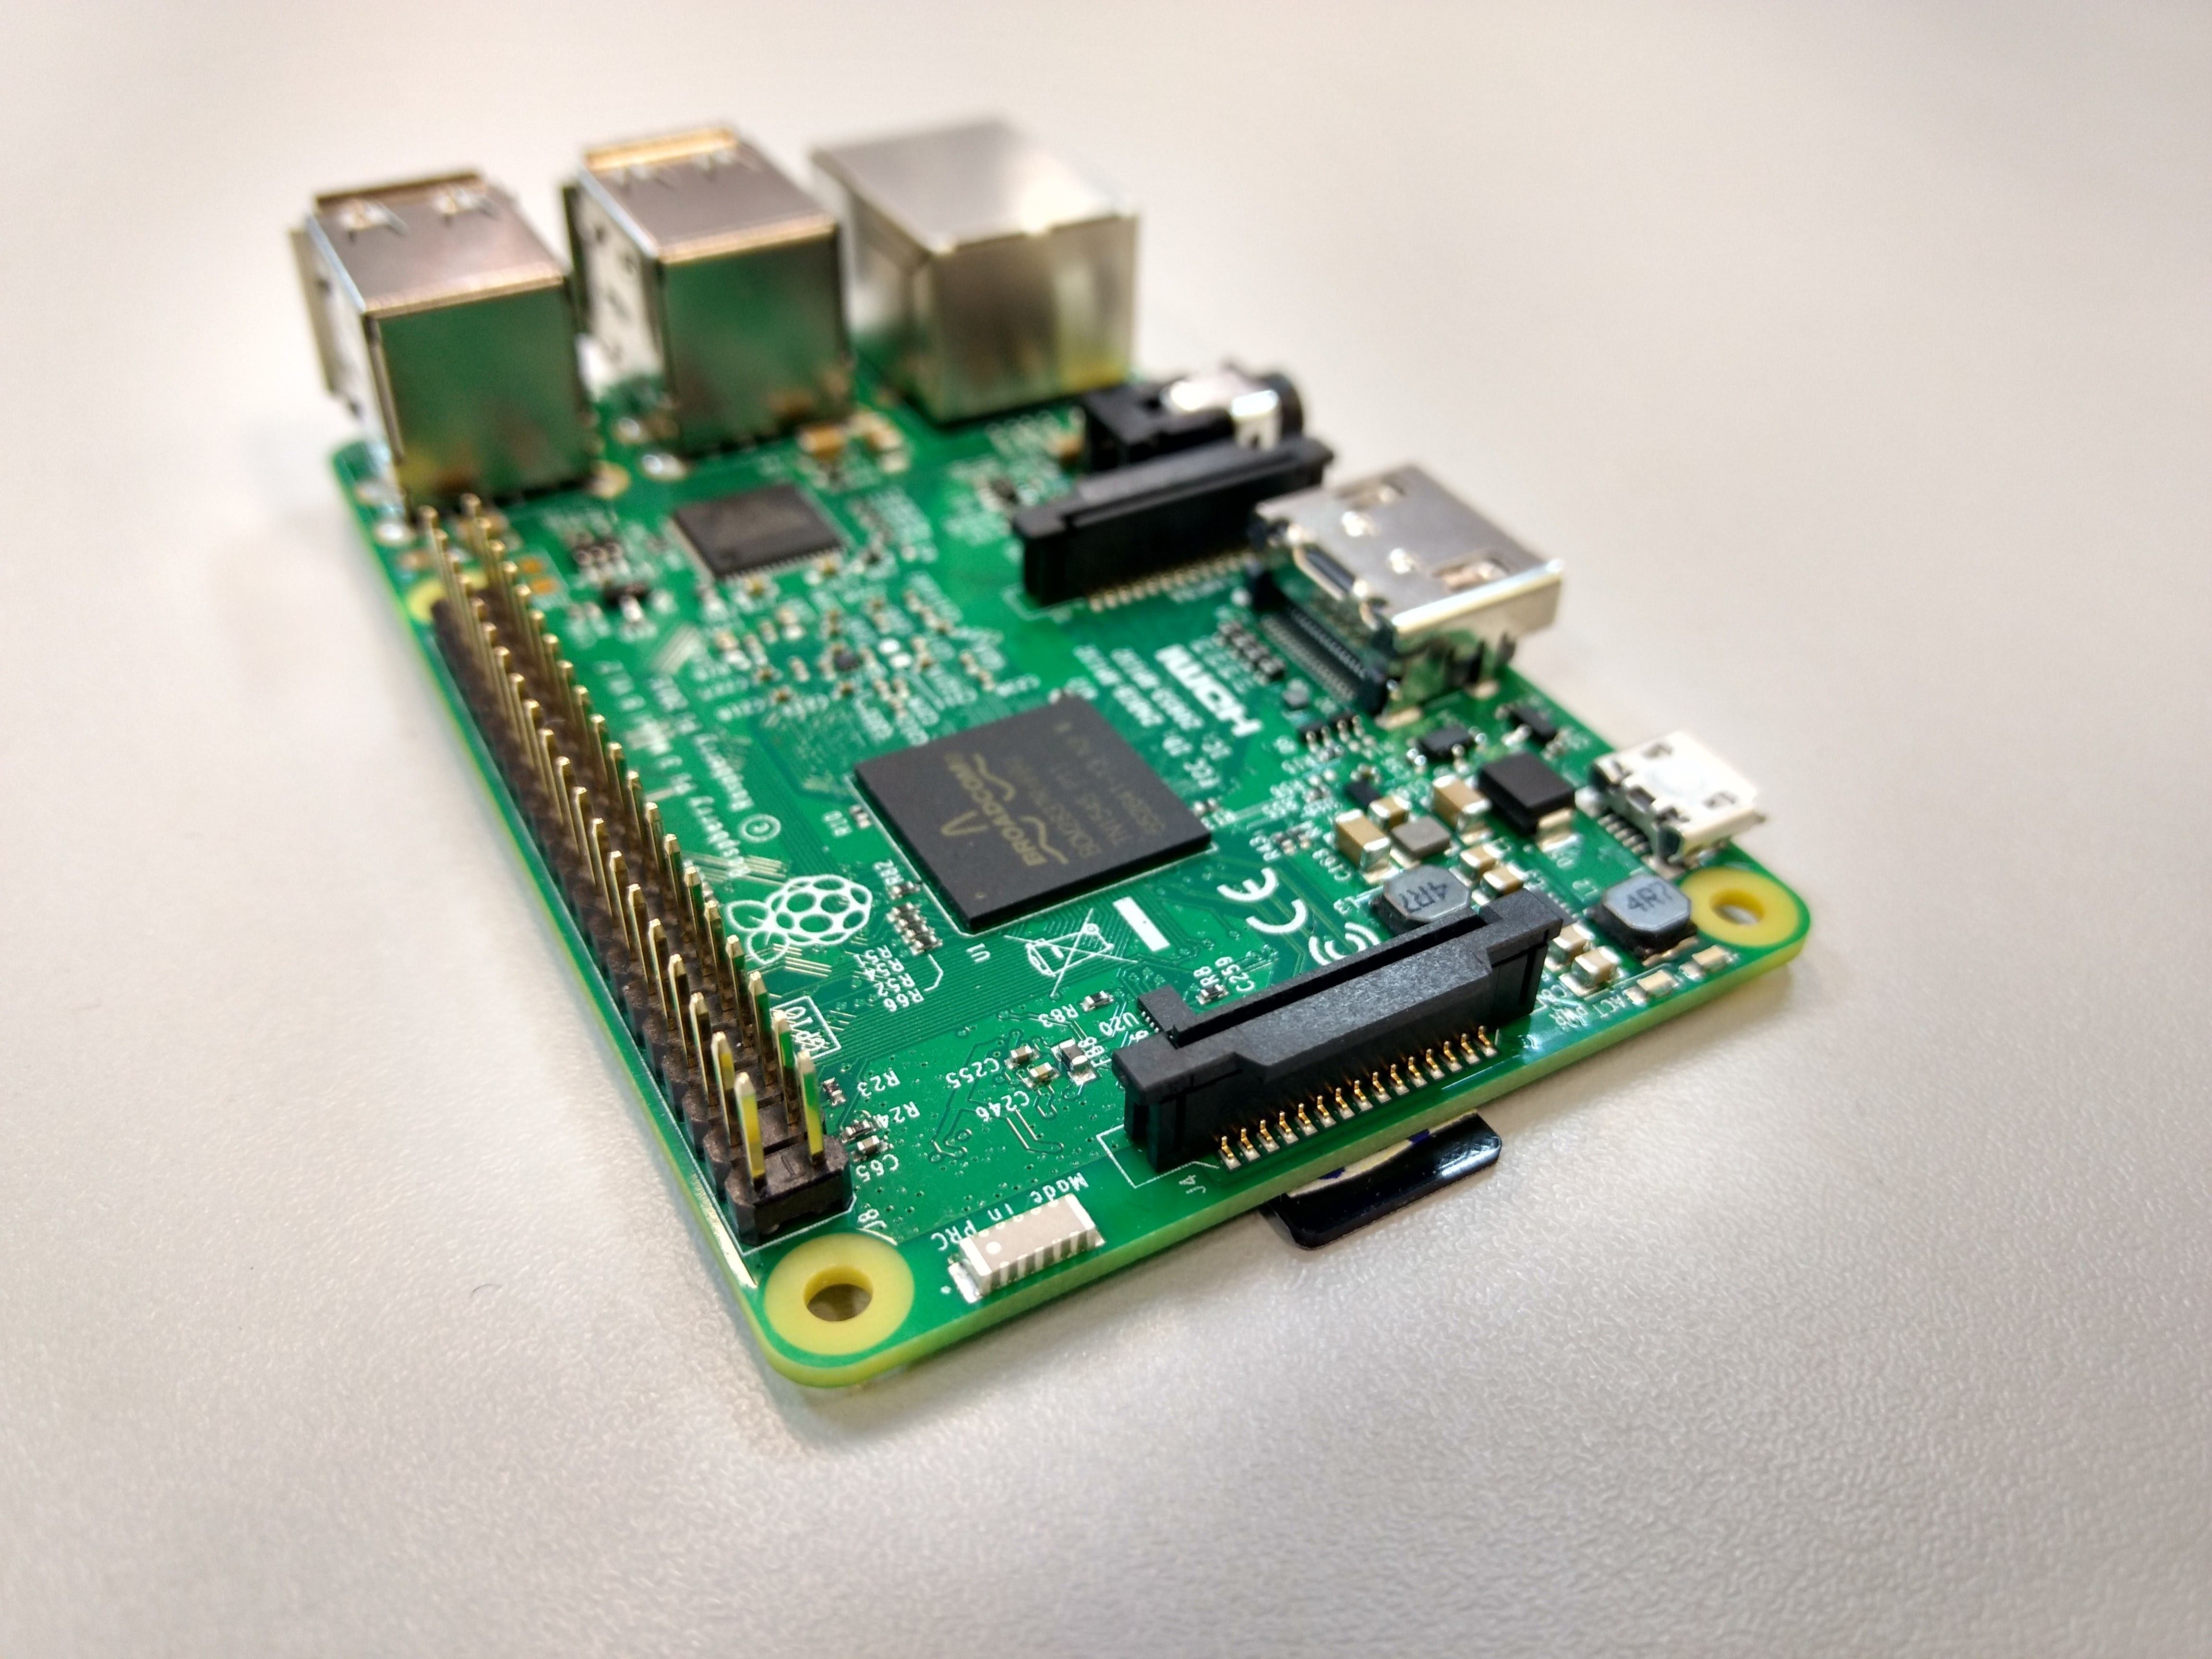
\includegraphics[width=1\textwidth]{040-plataformas/RPi-Wi-Fi-dongles/rpi-onboard.jpg}
	\end{center}
	\legend{Fonte: Elaborada pelo autor}
\end{figure}

Concomitantemente com o desenvolvimento e testes com ESP8266, foi desenvolvido
software para transformar o Raspberry Pi em uma plataforma para hospedar o
sensor. Sua principal diferença é o sistema operacional linux (inexistente no
ESP8266) que favorece o Raspberry e o alto custo que o desfavorece. Em média no
exterior o Raspberry Pi é vendido por USD \$ 35,00 (Raspberry Foundation)
e no Brasil por R\$ 250,00 (Mercado Livre).

As vantagens de ter um computador moderno completo sobrepõem seu custo em muitas
vezes. Dentre as quais destacamos a interface "amigável" com usuário devido ao
sistema operacional oferecendo maior nível de abstração (bastando apenas alguns
comandos para acessá-los realizar tarefas complexas), comunidade \emph{open
source} e o poder computacional.

Além deste recurso a nível de sistema, a comunidade e número de projetos "faça
você mesmo" é muito maior que a do ESP8266, devido a sua simplicidade em
conectar-se a um monitor e construir protótipos e aplicações.

**Alimentação**

O Raspberry é ligado por uma fonte de 2A, 5V e 10W através de uma entrada micro
USB. Para ligá-la, foi adquirido uma fonte USB tipo A para iPad, pois além de
poder desconectar o cabo da fonte, facilitando a manutenção, fornece a
quantidade exata de amperagem que o computador precisa. A primeira aquisição foi
de um carregador de \emph{smartphone} que não forneceu os amperes necessários.

Figura x.x - Carregador USB
![](carregador-ipad.jpg)

**Sistema Operacional**

O Raspberry Pi comporta sistemas operacionais que são carregados através no
micro cartão SD. Alguns exemplos de sistemas compatíveis: Archlinux, OpenELECE,
Raspbian, Risc, Pidora, Kali Linux, Windows 10 IoT, entre outros. Para este
trabalho, foi utilizado o Raspbian.

Figura X.X - Raspbian
![](raspbian.png)
Fonte: Elaborada pelo autor.

**Conclusão sobre Raspberry Pi**

O Raspberry foi adotado como o sensor para detectar os dispositivos. O modo
promíscuo conseguiu ser acessado através de adaptador/módulo USB Wi-Fi. Mais
detalhes sobre a construção e adoção deste computador serão apresentados no
capítulo "Construção".

**Comparativo RPi X ESP8266**

Em comparação com o ESP8266, o Raspberry Pi compensou seu preço mais caro devido
a facilidade de programação e acesso aos seus recursos e integração e acesso a
recursos externos. Além disso, foi possível chegar ao modo promíscuo facilmente
através do Bash e do sistema operacional. A seguir, uma tabela comparando as
principais características do RPi e do módulo ESP12F.

Figura X.X - RPi x ESP12F
![](rpi-esp.png)
Fonte: Elaborada pelo autor.
